\section{Finding a solution}

The software presented in the previous section, came a long way from the prototype 
that preceded it, however the complete solution to bringing circuit awareness and 
management into production is still under development.

\subsection{Difficulties in using NSI}

Although NSI is now the most popular implementation that promises to provide 
circuits in a production environment, it comes nonetheless with a few limitations.

\begin{description}[style=unboxed,leftmargin=0cm]
  \item[Provides a layer 2 circuit:] In contrast to Dynes which provided Layer 3 
  circuits between two servers, NSI only provides a Layer 2 circuit. This means that 
  the transfer backends used in PhEDEx cannot directly use it. A Layer 3 path 
  has to be created on top of the Layer 2 circuit. Constructing such a path means 
  having privileged access to the site's network infrastructure - something that is 
  not trivial, especially with the start of LHC operations in 2015.
  \item[Circuit ends at the border router:] The Layer 2 path doesn't end at the storage 
  servers, nor does it end at the storage farm's router. The Layer 3 path needs to 
  be created not just on top of the circuit, but also from the border routers to the 
  storage 
  \item[Guarantee bandwidth is not supported by all providers:] The motivation of using 
  circuits in PhEDEx is two fold: provide more deterministic transfer times and 
  provide a way of privileging select traffic. If even a single circuit provider 
  involved in an inter-domain transfer doesn't guarantee the bandwidth which PhEDEx 
  asks for, then the advantages of using circuits in PhEDEx may be lost.
  \item[NSI adoption is still limited:] Even though NSI has a lot more support from 
  big network providers, adoption into production is still limited. 
\end{description}

\subsubsection{Difficulties in dealing with Layer2 circuits}

Since the transfer backends can't directly used Layer 2 circuits, a Layer 3 path needs to be 
established between the storage servers, or at least between the routers of the storage farms.

Establishing a Layer 3 path, is non-trivial since:
\begin{description}[style=unboxed,leftmargin=0cm]
  \item[It requires topology and routing info:] PhEDEx is a very high-level software. It only 
  knows about its transfer queue, name of sites, and name and sizes of datasets, blocks and 
  files. Its monitoring information is limited and the PFNs involved in the transfer don't 
  point directly to the file replica used in the data movement. 
  \item[Direct access to the site's network:] Perhaps the biggest challenge in establishing 
  a Layer 3 path is the fact that one requires direct access to the site's network infrastructure.
  Doing live modifications of the routing information on any production network is controversial 
  enough, even without thinking of that that infrastructure is critical to the success of LHC's 
  Run 2.
\end{description}

\subsection{Difficulties in using FTS/SRM}

Not all difficulties in coming up with a solution stem from using NSI as a circuit backend.
FTS/SRM and gridFTP are the most popular protocols involved in data transfer and naturally 
any solution that we propose should at the very least work with them. 

The problem here is best described in Figure \ref{fig:SURL-to-TURLs}.

In a (PhEDEx) file transfer, two PFNs are always involved: the source and destination PFNs. 
Ideally, these PFNs should directly point to the physical storage location 
of the files that need to be transferred. With FTS and SRM, the PFNs don't reflect that. 
They are only Storage URLs (SURL) and they point to the storage farm's FTS server. 
In order to get the exact location of the file, FTS needs to pick a file replica from one 
of the storage elements. Only once that's done, and the SURL is transformed into a Transfer 
URL (TURL), can a transfer begin.

This is particularly important because the actual servers involved in the transfer, 
must be known in order to establish circuits between them.

\begin{figure}[h]
  \centering
  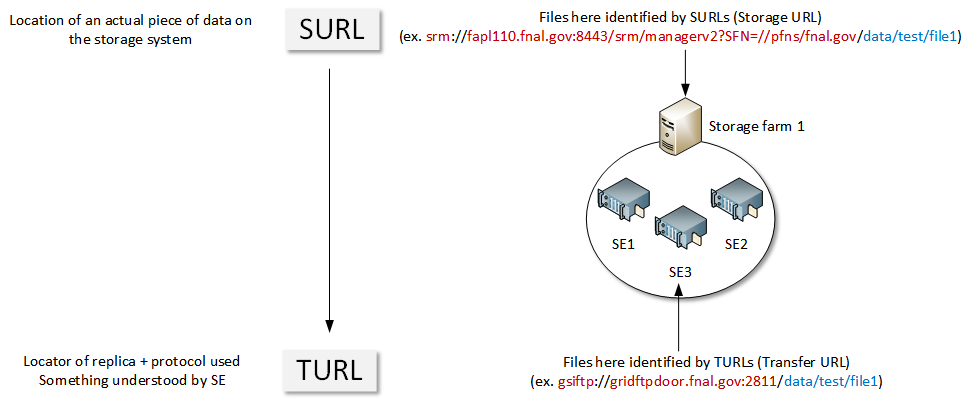
\includegraphics[width=0.95\textwidth]{Figures/TURL_to_SURL.png}
  \caption{View of PhEDEx-only transfers on both the shared and dedicated path}
  \label{fig:SURL-to-TURLs}
\end{figure} 

\subsection{Proposed solution}

Ideally, any proposed solution should:
\begin{itemize}
	\item Work in a multiple VO environment
	\item Try and deal with privileged and unprivileged traffic on the same path
	\item Work with FTS/SRM and gridFTP
	\item Be as un-intrusive into the site's operations as possible
\end{itemize}

The solution which was put forward is presented in Figures \ref{fig:global-solution-view} 
and \ref{fig:zoom-solution-view}. 

\begin{itemize}
	\item The ResourceManager is used to request a Layer 2 circuit between the border routers
	of sites A and B. The request can come from either PhEDEx or any external application that 
	uses our REST API.
	\item Once the Layer 2 circuit is up:
		\begin{itemize}
			\item A wrapper is used to retrieve all the storage servers (looking in the TURLs) 
			involved in the transfer. This information is passed to an OpenFlow controller
			\item The ResourceManager informs the OpenFlow controller that a new Layer 2 path 
			is available.
		\end{itemize}
	\item The OpenFlow controller adds routing information in all the OpenFlow switches, 
	directing all traffic coming from servers involved in the transfer, onto the newly created 
	circuit
\end{itemize}

\begin{figure}[h]
  \centering
  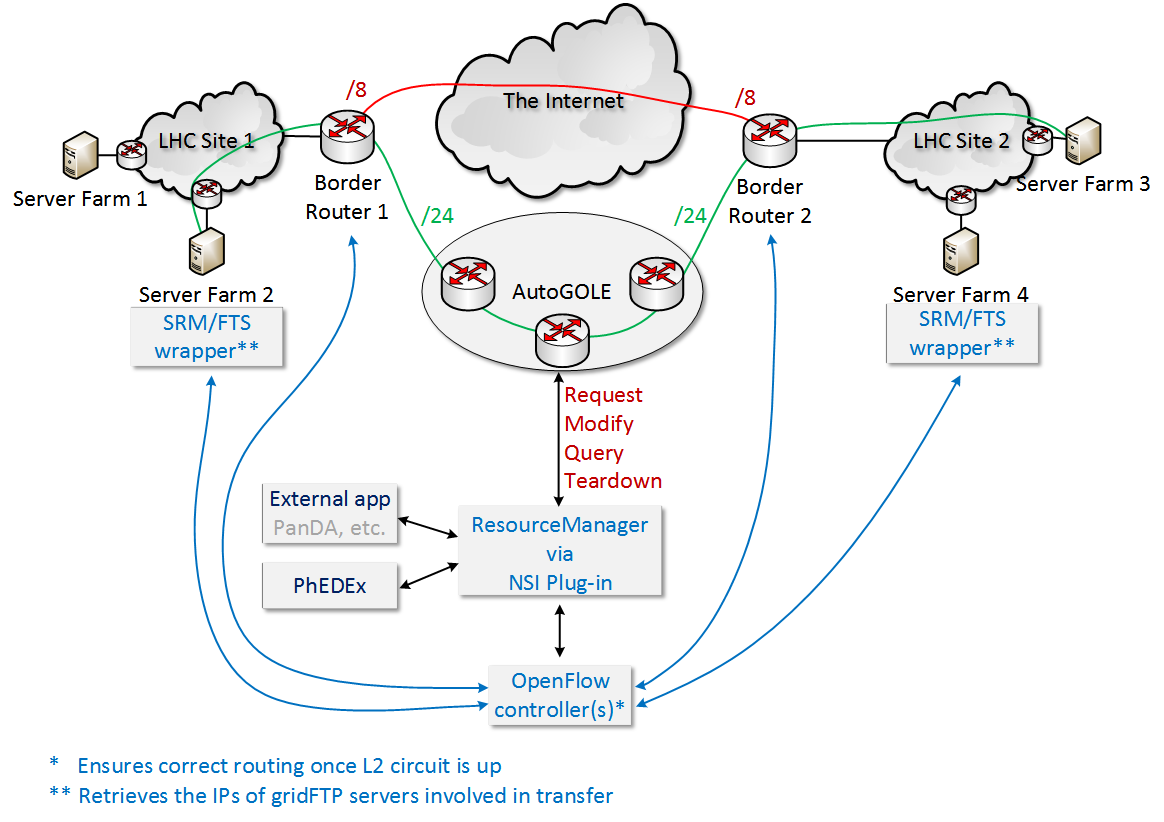
\includegraphics[width=0.95\textwidth]{Figures/Proposed_solution-global_view.png}
  \caption{Global view of our proposed solution}
  \label{fig:global-solution-view}
\end{figure} 

\begin{figure}[h]
  \centering
  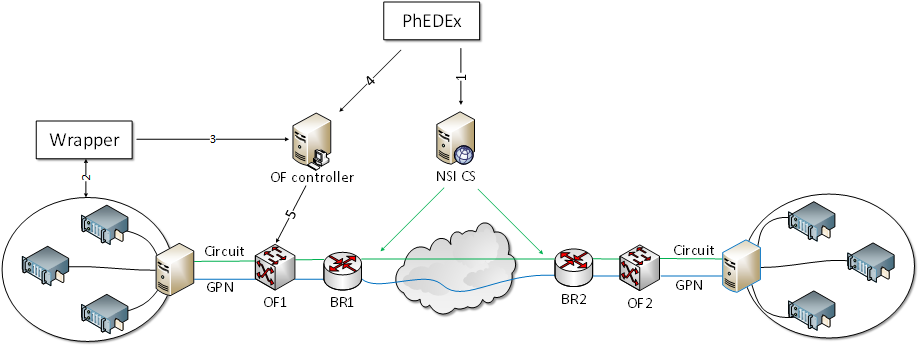
\includegraphics[width=0.95\textwidth]{Figures/Proposed_solution-zoom_view.png}
  \caption{In depth view of our proposed solution}
  \label{fig:zoom-solution-view}
\end{figure} 

